\documentclass[12pt,letterpaper]{report}
\usepackage{fontspec}\setmainfont{TeX Gyre Termes}
\usepackage{polyglossia}\setdefaultlanguage{spanish}
\usepackage[left=4cm,right=3cm,top=3cm,bottom=3cm]{geometry}
\usepackage{longtable,array,booktabs,graphicx,float,hyperref}
\hypersetup{hidelinks}
\usepackage{setspace}\onehalfspacing
\setlength{\parindent}{0pt}\setlength{\parskip}{6pt}
\begin{document}
\setcounter{chapter}{2}\setcounter{section}{6}
\section{Seguridad}
% Insertar bajo el encabezado 2.7 Seguridad.
% Este archivo incluye los encabezados 2.7.1, 2.7.2 y 2.7.3.

\subsection{Autenticación y gestión de sesiones}

El acceso al panel web se realiza mediante correo electrónico y contraseña
a través de \texttt{/api/v1/login}. El servidor consulta la cuenta y exige que
se encuentre activa y no esté eliminada. La contraseña recibida se compara
con el hash almacenado mediante bcrypt con costo 12; las contraseñas no se almacenan en
texto plano. Cuando la cuenta no cumple las condiciones o la contraseña no
coincide, se devuelve una respuesta HTTP 401 con un mensaje genérico, sin
indicar cuál de las credenciales es incorrecta. La ruta de inicio de sesión
limita las solicitudes a diez intentos por minuto mediante el middleware
de control de frecuencia; al exceder el límite responde con HTTP 429.

Después de una autenticación válida, el servidor emite un token JWT firmado
con el algoritmo HS256 y una vigencia de ocho horas. El token identifica al
usuario e incluye la versión de su sesión. En cada petición protegida, el
middleware comprueba la firma y la expiración, consulta nuevamente la cuenta
y compara la versión del token con \path{version_sesion}. También verifica
que el usuario permanezca activo y pertenezca a la clínica solicitada.

La interfaz conserva el token en \texttt{sessionStorage}, bajo la clave
\texttt{clinica-token}. El interceptor HTTP lo incorpora al encabezado
\texttt{Authorization} utilizando el esquema Bearer. Este almacenamiento
está asociado a la sesión de la pestaña y no se utiliza
\texttt{localStorage} para conservar el token. Sin embargo,
\texttt{sessionStorage} es accesible desde JavaScript: no equivale a una
cookie \texttt{HttpOnly} ni proporciona protección por sí solo frente a
la ejecución de scripts maliciosos.

La implementación no utiliza tokens de refresco ni renovación automática.
Cuando el JWT vence, la API responde con HTTP 401; el interceptor elimina
el token almacenado y dirige al usuario a la pantalla de acceso para que
inicie sesión nuevamente. Esta conducta también se aplica cuando el
servidor detecta una sesión invalidada.

El cierre de sesión llama a \path{/api/v1/logout}. El servidor incrementa
\path{version_sesion}, de modo que los tokens previamente emitidos para
esa cuenta dejan de ser válidos en las siguientes solicitudes, incluso
si todavía no han alcanzado su fecha de expiración. Después de recibir la
confirmación, la interfaz limpia el almacenamiento de sesión y vuelve al
inicio de sesión. Esta invalidación afecta a las sesiones anteriores de
la cuenta, no solamente a la pestaña que solicita el cierre. El cambio y
el restablecimiento de contraseña también incrementan la versión de sesión.

La clave de firma del JWT y las credenciales de base de datos y almacenamiento
se obtienen desde variables de entorno del backend. El archivo local
\texttt{backend/.env} está excluido del repositorio y estas credenciales
no se incorporan al código del frontend.

\subsection{Autorización por roles o perfiles}

La autorización se aplica en dos niveles. En la interfaz se muestran las
opciones y acciones disponibles según la sesión. En el servidor se
comprueban los permisos de cada operación y el alcance de los registros
solicitados. La comprobación del backend es necesaria aunque se invoque
directamente una ruta HTTP sin utilizar el menú de la aplicación.

Las asociaciones de usuarios y roles se conservan en
\texttt{roles\_modelos}; los permisos de cada rol se almacenan en
\texttt{permisos\_roles}, y los permisos directos de usuarios en
\texttt{permisos\_modelos}. El servidor recupera esta información al
validar las solicitudes. Los permisos distinguen operaciones como lectura,
creación, actualización y eliminación. Los perfiles internos tienen las
siguientes responsabilidades:

\begin{itemize}
  \item \textbf{Administrador:} administra cuentas, roles y permisos y
  supervisa los registros del sistema dentro de las clínicas a las que
  pertenece. El rol interno \texttt{Super Admin} satisface las comprobaciones
  generales de permisos; las rutas de administración utilizan además la
  comprobación \texttt{requireAdmin}.

  \item \textbf{Odontólogo:} gestiona los pacientes que tiene asignados
  y sus solicitudes radiográficas, de acuerdo con los permisos otorgados.
  Las consultas de pacientes y radiografías comprueban la relación de
  asignación, y las consultas de citas y recetas incorporan también el
  identificador del profesional. No dispone de administración de cuentas
  y permisos por el hecho de tener el rol de odontólogo.

  \item \textbf{Recepcionista:} consulta, registra y actualiza datos
  administrativos de pacientes; consulta odontólogos y horarios; gestiona
  citas y asigna pacientes a profesionales. El servidor limita los campos
  visibles y modificables y no le concede acceso a radiografías,
  antecedentes clínicos, recetas o administración de cuentas. La
  revocación de una asignación está reservada al administrador.
\end{itemize}

CERPAX no es un perfil con inicio de sesión en el panel. Su acceso se limita
al portal de entrega mediante un token temporal vinculado a una solicitud.
La validación exige que el enlace esté vigente, no haya sido revocado ni
utilizado y corresponda a una solicitud pendiente. El token se conserva
como hash en la base de datos. Un enlace inválido o no disponible genera
HTTP 410. El paciente se representa como registro clínico y no como actor
de acceso al panel. El servidor rechaza su inicio de sesión incluso si tiene
contraseña válida y rechaza los JWT anteriores de cuentas con el único rol
\texttt{Patient}. Compartir la tabla \texttt{usuarios} permite reutilizar los
datos personales; no concede autorización para ingresar al sistema.

Para el aislamiento entre clínicas, el servidor verifica que el valor del
encabezado \texttt{X-Company-ID} pertenezca a las clínicas autorizadas del
usuario. Posteriormente incorpora ese alcance en las consultas. Los
permisos insuficientes generan HTTP 403; algunos accesos a registros fuera
del alcance autorizado responden con HTTP 404 para no revelar su existencia.
El acceso local de desarrollo está condicionado a la configuración y a
la dirección de conexión; se deshabilita cuando el entorno es producción.

Las cuentas internas se crean desde la administración. Un nuevo registro
de odontólogo recibe el rol \texttt{Doctor}; un paciente recibe
\texttt{Patient} y no obtiene acceso al panel. Las cuentas administrativas
creadas sin rol no pueden iniciar sesión hasta que el administrador les asigne
un perfil interno. Solo el administrador puede modificar estas asociaciones
mediante \path{/api/v1/users/:id/access}. No existe registro público que
conceda privilegios administrativos.

\begingroup
\footnotesize
\setlength{\tabcolsep}{3pt}
\renewcommand{\arraystretch}{1.2}
\begin{longtable}{@{}>{\raggedright\arraybackslash}p{.42\linewidth}>{\raggedright\arraybackslash}p{.11\linewidth}>{\raggedright\arraybackslash}p{.15\linewidth}>{\raggedright\arraybackslash}p{.15\linewidth}>{\raggedright\arraybackslash}p{.10\linewidth}@{}}
\caption{Autorización de las rutas principales según el perfil}\label{tab:matriz-rutas}\\
\toprule
\textbf{Método y ruta} & \textbf{Admin.} & \textbf{Odontólogo} & \textbf{Recepción} & \textbf{CERPAX}\\\midrule
\endfirsthead
\toprule
\textbf{Método y ruta} & \textbf{Admin.} & \textbf{Odontólogo} & \textbf{Recepción} & \textbf{CERPAX}\\\midrule
\endhead
\bottomrule\endlastfoot
POST \path{/api/v1/login} & Sí & Sí & Sí & No\\
GET/POST/PUT/DELETE \path{/api/v1/cuentas} y \path{/api/v1/cuentas/:id} & Sí & No & No & No\\
GET/POST/PUT/DELETE \path{/api/v1/roles} y \path{/api/v1/roles/:id} & Sí & No & No & No\\
GET/PUT \path{/api/v1/users/:id/access} & Sí & No & No & No\\
GET/POST/PUT \path{/api/v1/pacientes} y \path{/api/v1/pacientes/:id} & Sí & Ámbito propio & Datos administrativos & No\\
DELETE \path{/api/v1/pacientes/:id} & Sí & Asignados & No & No\\
GET \path{/api/v1/odontologos} y \path{/api/v1/horarios} & Sí & Sí & Sí & No\\
POST/PUT/DELETE \path{/api/v1/odontologos/:id} & Sí & No & No & No\\
GET \path{/api/v1/citas} y \path{/api/v1/citas/:id} & Sí & Ámbito propio & Sí & No\\
POST/PUT/DELETE \path{/api/v1/citas} y \path{/api/v1/citas/:id} & Sí & No & Sí & No\\
GET/POST \path{/api/v1/radiographs} & Sí & Asignados & No & No\\
POST \path{/api/v1/radiographs/:id/access} & Sí & Asignados & No & No\\
GET \path{/api/v1/radiographs/:id/file} & Sí & Asignados & No & No\\
GET/POST \path{/api/v1/patient-assignments} & Sí & No & Sí & No\\
DELETE \path{/api/v1/patient-assignments/:patient/:doctor} & Sí & No & No & No\\
GET \path{/api/v1/radiography-audit} & Sí & No & No & No\\
POST \path{/api/v1/external/radiographs/access}, \path{/upload-url} y \path{/upload-complete} & Token temporal & Token temporal & Token temporal & Token temporal\\
\end{longtable}
\noindent\textit{Fuente: elaboración propia a partir del código y las migraciones.}
\endgroup

La matriz corresponde a los permisos predeterminados. Las rutas de modificación
de cuentas, roles y asignación de roles exigen administrador, incluso si se
concede un permiso directo de lectura de cuentas a un odontólogo. La creación
usa la ruta de colección; la actualización y eliminación requieren el
identificador. Las rutas externas comparten el prefijo
\path{/api/v1/external/radiographs}; requieren un token temporal vigente,
independientemente de que quien posea el enlace disponga de una cuenta interna.
El paciente no puede autenticarse ni utilizar las rutas internas.

\subsection{Validación de entradas y protección}

La interfaz utiliza controles de formulario para orientar la captura de
datos, como campos obligatorios, tipos de entrada y opciones disponibles.
El backend realiza su propia validación, ya que los datos pueden enviarse
sin pasar por la interfaz. Las reglas comprueban campos permitidos,
identificadores numéricos, formatos de correo, longitudes máximas,
valores de listas, números finitos y estructuras JSON. Las validaciones
clínicas comprueban fechas y horarios y rechazan intervalos inconsistentes
y superposiciones de citas.

Las operaciones con PostgreSQL utilizan consultas parametrizadas: los
valores recibidos se envían separados del texto SQL mediante marcadores
como \texttt{\$1} y \texttt{\$2}. Los nombres de módulos y campos se
resuelven desde el catálogo y los metadatos permitidos, y los identificadores
SQL se validan antes de incorporarse a las consultas dinámicas. Estas
medidas reducen el riesgo de inyección SQL sin atribuir a una consulta
parametrizada la validación de nombres de tablas o columnas.

Para las radiografías se admiten PDF, PNG, JPEG y WebP con un tamaño máximo
de \mbox{50 MiB}. En la carga directa a Supabase Storage, la API valida el
nombre, la extensión, el tipo MIME y el tamaño declarado antes de emitir
la URL firmada. Al confirmar, comprueba la existencia del objeto, su tamaño
y la correspondencia de su ruta con el acceso temporal. En las rutas de
carga multipart que reciben el archivo en el servidor se utiliza Multer
para limitar el tamaño y se identifica el formato a partir de la firma
binaria. La validación de metadatos de la carga directa no se presenta como
una inspección completa del contenido del archivo.

Los objetos radiográficos se mantienen en almacenamiento privado. Antes
de abrir un archivo, la API vuelve a comprobar la autorización del usuario
sobre la solicitud. Las operaciones que completan una entrega utilizan
transacciones y restricciones de unicidad para conservar la coherencia
entre la solicitud, el archivo y el acceso utilizado.

Express aplica los encabezados de seguridad de Helmet y una política de
seguridad de contenido que restringe los orígenes de scripts, imágenes y
conexiones. La API comprueba el encabezado de origen cuando está presente
y rechaza los orígenes no permitidos con HTTP 403. Este control complementa
la autenticación y no la sustituye. El procesamiento de cuerpos JSON está
limitado a \mbox{2 MiB}, de forma independiente del límite de archivos.

El manejador centralizado de errores devuelve respuestas JSON y evita
exponer consultas internas, contraseñas o cadenas de conexión. Se utiliza
HTTP 400 para errores de formato de la petición, HTTP 401 para autenticación,
HTTP 403 para autorización, HTTP 409 para conflictos y HTTP 422 para
validaciones de datos, según la ruta y la condición detectada. Los errores
internos generan un mensaje genérico con HTTP 500. Las respuestas de la
API incluyen \texttt{Cache-Control: no-store} para evitar su almacenamiento
en cachés HTTP.

Estas medidas se respaldan con pruebas del backend que comprueban ausencia
de sesión, permisos insuficientes, acceso entre clínicas, pacientes no
asignados, enlaces vencidos o revocados y validación de archivos y datos.
Los resultados obtenidos y sus evidencias se presentan en la sección de pruebas.

\section{Pruebas}
% Insertar bajo 2.8 Pruebas; requiere longtable,array,booktabs,graphicx,float,hyperref.
Las pruebas verifican los cuatro requisitos prioritarios: autenticación
(RF-01), pacientes (RF-02), solicitudes radiográficas (RF-03) y acceso
temporal por enlace o QR (RF-04). Se utilizan caminos correctos y errores,
con datos sintéticos, comprobando el estado HTTP y las reglas de acceso.

\subsection{Entorno y ejecución}

Las pruebas automatizadas ejecutan el backend real de Express y sus
migraciones SQL sobre PostgreSQL embebido mediante PGlite. Supertest realiza
solicitudes HTTP y Playwright verifica el acceso desde el navegador y genera
evidencias. Este entorno está aislado de los pacientes y archivos reales.
La prueba local de archivos utiliza la ruta multipart y contenido en la base
de prueba; no acredita la carga directa de producción en Supabase Storage.

La ejecución del 11/10/2026 a las 22:20:56 (hora de Bolivia)
registró 31 pruebas, 31 aprobadas y 0 fallidas, sin omitidas.
El escenario adicional de navegador se aprobó y verificó 15
respuestas HTTP. El archivo de seguridad específico registra 22
comprobaciones HTTP; estos conteos describen distintos niveles y no deben sumarse
como si fueran casos independientes.

Los comandos reproducibles son \texttt{npm run test:report} y
\texttt{npm run test:e2e -w backend -- security.spec.js}.
El reporte completo se conserva en
\path{evidencia/reporte-pruebas-e3.txt}; las respuestas resumidas se encuentran
en \path{evidencia/seguridad-http.json} y
\path{evidencia/evidencias-navegador.json}. Ninguno incluye contraseñas ni JWT.

\subsection{Casos ejecutados}

\begingroup
\footnotesize
\setlength{\tabcolsep}{3pt}
\renewcommand{\arraystretch}{1.2}
\begin{longtable}{@{}>{\raggedright\arraybackslash}p{.09\linewidth}>{\raggedright\arraybackslash}p{.24\linewidth}>{\raggedright\arraybackslash}p{.21\linewidth}>{\raggedright\arraybackslash}p{.27\linewidth}>{\raggedright\arraybackslash}p{.11\linewidth}@{}}
\caption{Casos de prueba ejecutados y resultados observados}\label{tab:pruebas-reales}\\
\toprule
\textbf{ID}&\textbf{Escenario}&\textbf{Esperado}&\textbf{Obtenido y evidencia}&\textbf{Estado}\\\midrule
\endfirsthead
\toprule
\textbf{ID}&\textbf{Escenario}&\textbf{Esperado}&\textbf{Obtenido y evidencia}&\textbf{Estado}\\\midrule
\endhead
\bottomrule\endlastfoot
CP-01 & RF-01: credenciales válidas & HTTP 200 y JWT & HTTP 200; EV-01; Figura~\ref{fig:prueba-200} & Aprobado \\
CP-02 & RF-01: contraseña incorrecta & HTTP 401, mensaje genérico & HTTP 401; EV-02 & Aprobado \\
CP-03 & Sin JWT en pacientes & HTTP 401 & HTTP 401; EV-03; Figura~\ref{fig:prueba-401} & Aprobado \\
CP-04 & Odontólogo consulta cuentas & HTTP 403 & HTTP 403; EV-08; Figura~\ref{fig:prueba-403} & Aprobado \\
CP-05 & RF-02: paciente sin campos obligatorios & HTTP 422 & HTTP 422; EV-04; Figura~\ref{fig:prueba-422} & Aprobado \\
CP-06 & RF-02: crear, consultar, actualizar y eliminar paciente & 201, 200, 200, 200; posterior 404 & Códigos coincidentes; SEG-04 a 06 y SEG-21 a 22 & Aprobado \\
CP-07 & Paciente ajeno al odontólogo & HTTP 404 & HTTP 404; SEG-11 & Aprobado \\
CP-08 & RF-03: crear solicitud de paciente asignado & HTTP 201 y asociación persistida & HTTP 201; EV-11; verificación SQL en radiography.test.js & Aprobado \\
CP-09 & RF-03: solicitar estudio sin asignación & HTTP 404 & HTTP 404; EV-09 & Aprobado \\
CP-10 & RF-04: generar enlace y QR & HTTP 201, URL y PNG del QR & HTTP 201; EV-12 y EV-13 & Aprobado \\
CP-11 & RF-04: validar acceso vigente & HTTP 200, datos mínimos & HTTP 200; EV-15 & Aprobado \\
CP-12 & RF-04: reutilizar enlace revocado & HTTP 410 & HTTP 410; EV-14 & Aprobado \\
CP-13 & Enlace vencido y carga repetida & HTTP 410 en ambos casos & HTTP 410; radiography.test.js & Aprobado \\
CP-14 & Carga multipart local y consulta protegida & HTTP 201 y 200; solicitud completada & Códigos coincidentes; radiography.test.js & Aprobado \\
CP-15 & Archivo con contenido o extensión inválidos; exceso de tamaño & 422, 422 y 413 & Códigos coincidentes; radiography.test.js & Aprobado \\
CP-16 & Paciente intenta ingresar con contraseña válida o JWT anterior & HTTP 401; sin token nuevo & HTTP 401; SEG-16 y SEG-17 & Aprobado \\
CP-17 & JWT alterado, vencido o reutilizado después de logout & HTTP 401 & HTTP 401; SEG-13, SEG-18 y SEG-20 & Aprobado \\
CP-18 & Odontólogo usa otra clínica & HTTP 403 & HTTP 403; SEG-14 & Aprobado \\
CP-19 & Permiso directo de cuentas concedido a odontólogo & HTTP 403 también en ruta anterior & HTTP 403; SEG-15 & Aprobado \\
CP-20 & Recepcionista intenta acceder a radiografías y datos clínicos & HTTP 403 y omisión de campos sensibles & Comprobado; receptionist.test.js & Aprobado \\
\end{longtable}
\noindent\textit{Fuente: elaboración propia a partir de la ejecución automatizada.}
\endgroup

Los identificadores EV corresponden al informe de navegador y los SEG al
informe HTTP de seguridad. Los archivos de pruebas citados pertenecen a
\path{backend/test/}. Las filas agrupan operaciones relacionadas; el número
de filas no equivale al contador del ejecutor de Node.js.

\subsection{Evidencias}

Las siguientes capturas muestran respuestas reales del servidor de prueba
registradas por Playwright. Son capturas del informe de ejecución, con las
credenciales y los tokens omitidos, y no capturas del despliegue de Vercel.

\begin{figure}[H]
\centering
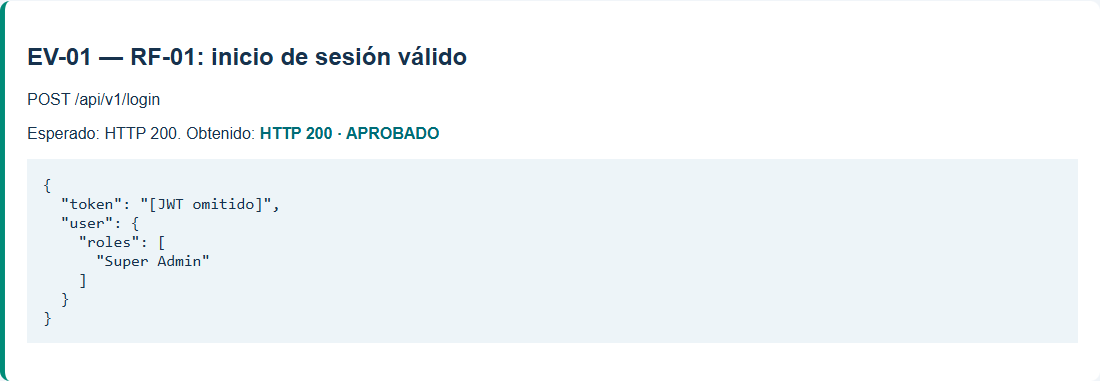
\includegraphics[width=\textwidth]{../../evidencia/http-200.png}
\caption{Inicio de sesión autorizado, CP-01. Fuente: ejecución propia en entorno local.}
\label{fig:prueba-200}
\end{figure}

\begin{figure}[H]
\centering
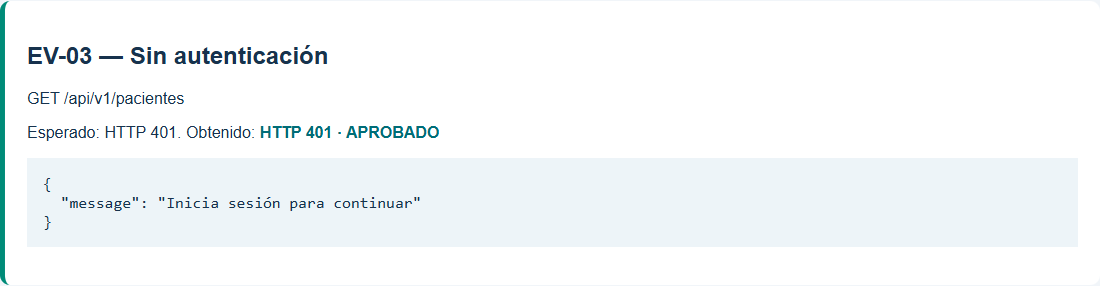
\includegraphics[width=\textwidth]{../../evidencia/http-401.png}
\caption{Acceso a pacientes sin JWT, CP-03. Fuente: ejecución propia en entorno local.}
\label{fig:prueba-401}
\end{figure}

\begin{figure}[H]
\centering
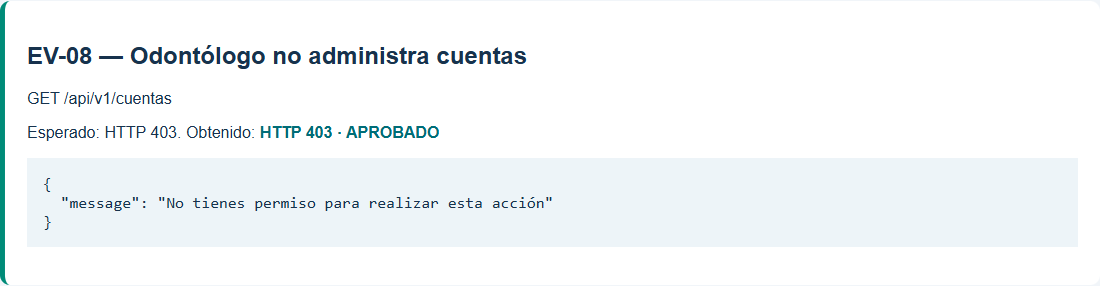
\includegraphics[width=\textwidth]{../../evidencia/http-403.png}
\caption{Consulta de cuentas por un odontólogo, CP-04. Fuente: ejecución propia en entorno local.}
\label{fig:prueba-403}
\end{figure}

\begin{figure}[H]
\centering
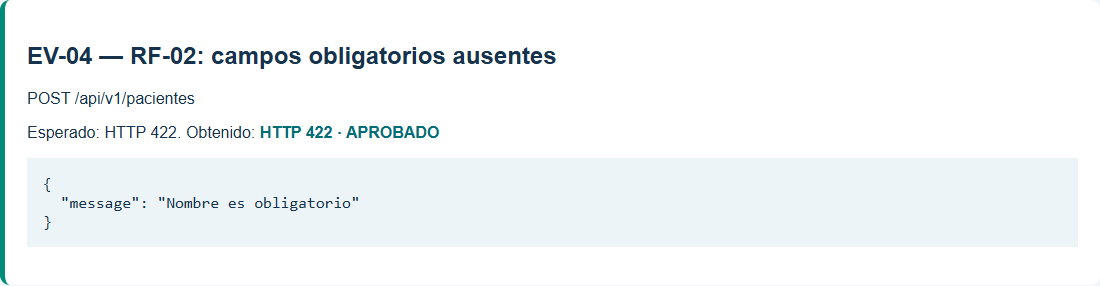
\includegraphics[width=\textwidth]{../../evidencia/http-422.png}
\caption{Registro de paciente sin campos obligatorios, CP-05. Fuente: ejecución propia en entorno local.}
\label{fig:prueba-422}
\end{figure}

El informe ampliado \path{evidencia/evidencias-seguridad.pdf} contiene las
15 respuestas del recorrido de navegador, incluidas la creación de la
solicitud, la generación del enlace y el rechazo del enlace revocado.

\subsection{Comprobaciones en producción y rendimiento}

En el despliegue de Vercel se realizaron comprobaciones de lectura:
la salud de la API respondió 200, el acceso a pacientes sin autenticación
respondió 401, el inicio de sesión respondió 200 y la consulta de solicitudes
radiográficas respondió 200. El detalle se conserva en
\path{evidencia/verificacion-despliegue.json}.

Se midieron diez consultas consecutivas autenticadas al listado de pacientes,
con página de quince registros y sin transferencias de archivos. La medición
incluye el tiempo observado por el cliente HTTP desde este equipo, la red y
la lectura de la respuesta JSON. No es una prueba de concurrencia ni de carga.

\begin{table}[H]\centering
\caption{Tiempos observados en consultas de pacientes en Vercel}
\begin{tabular}{rrr}\toprule
\textbf{Consulta}&\textbf{Estado HTTP}&\textbf{Tiempo (ms)}\\\midrule
1&200&349\\
2&200&214\\
3&200&209\\
4&200&251\\
5&200&219\\
6&200&222\\
7&200&208\\
8&200&320\\
9&200&213\\
10&200&217\\
\bottomrule\end{tabular}\end{table}
En esta muestra, 10 de 10 consultas respondieron en menos de tres
segundos, con un rango de 208 a 349 ms.
Se satisface el umbral de RNF-01 para esta operación y estas condiciones;
el resultado no se generaliza a todas las operaciones ni a usuarios concurrentes.

Las modificaciones de autorización y las nuevas rutas v1 documentadas en esta
revisión se verificaron localmente. El recorrido completo de creación,
enlace y entrega directa a Supabase Storage no se ejecutó en producción
durante esta revisión; las comprobaciones de lectura anteriores no lo
sustituyen. Antes de presentar la versión desplegada debe verificarse ese
recorrido sobre la misma revisión del código.

\end{document}
